\documentclass[11pt,twoside,a4paper]{report}
\usepackage[utf8]{inputenc}
\usepackage{amsmath}
\usepackage{graphicx}
\usepackage{gensymb}
\usepackage{tikz}
\usetikzlibrary{positioning}
\usepackage{geometry}
\geometry{
    left=2cm,
    right=0.64cm,
    top=0.64cm,
    bottom=2cm
}
\usepackage{multicol}
\setlength{\columnsep}{1cm}
\graphicspath{ {images/} }

\begin{document}

\chapter{Semester 2 Examination 2014-2015\\CZ4034 Information Retrieval}

\begin{multicols*}{2}

\section{Question 1}
\noindent \textbf{Question 1a} Explain the following concepts with examples

\noindent \textbf{(i)} Posting list: it is a list of document IDs that contain a specific dictionary term, and is used in inverted index. The posting list needs to be a variable size list so that new documents can be added easily to the list. 

\begin{center}
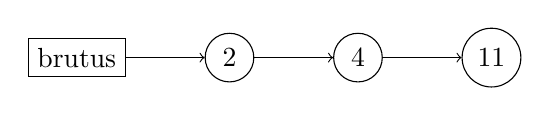
\begin{tikzpicture}[
squarenode/.style={rectangle, draw=black, thin},
roundnode/.style={circle, draw=black, thin},
]
%Nodes
\node[squarenode](brutus){brutus};
\node[roundnode](2)[right=of brutus]{2};
\node[roundnode](4)[right=of 2]{4};
\node[roundnode](11)[right=of 4]{11};

\draw[->](brutus.east) -- (2.west);
\draw[->](2.east) -- (4.west);
\draw[->](4.east) -- (11.west);
\end{tikzpicture}
\end{center}

\noindent \textbf{(ii)} Biword index: we use two consecutive words as dictionary pharases, instead of using unigram which treat each words as dictionary terms. For example, if we have the following sentence:
\begin{center}
\verb|I am a boy|
\end{center}
\noindent Then our dictionary phrases are: \verb|I am|, \verb|am a|, \verb|a boy|. \\

\noindent \textbf{(iii)} Stemming: Reduce terms to their “roots”, by crude chopping. For example:
\begin{itemize}
    \item automates automatic automation $\rightarrow$ automat
    \item democrats $\rightarrow$ democrat (noun)
    \item democratized $\rightarrow$ democratize (verb)
\end{itemize} 

\noindent \textbf{Question 1b} Given the entries of the permuterm index for the following terms: \verb|one|, \verb|two|, \verb|three|.

\noindent Answer: \verb|one$|, \verb|ne$o|, \verb|e$on|, \verb|$one|, \verb|two$|, \verb|wo$t|, \verb|o$tw|, \verb|$two|, \verb|three$|, \verb|hree$t|, \verb|ree$th|, \verb|ee$thr|, \verb|e$thre|, \verb|$three|\\

\noindent \textbf{Question 1c} Calculate the edit distance between \verb|work| and \verb|walk| by using Levenshtein distance algorithm

\begin{center}
\begin{tabular}{ | l | l  l  l  l  l |} 
    \hline
      &   & w & o & r & k \\
    \hline
      & 0 & 1 & 2 & 3 & 4 \\
    w & 1 & 0 & 1 & 2 & 3 \\
    a & 2 & 1 & 1 & 2 & 3 \\
    l & 3 & 2 & 2 & 2 & 3 \\
    k & 4 & 3 & 3 & 3 & \textbf{2} \\
    \hline
\end{tabular}
\end{center}

\noindent \textbf{Question 1d} Assume that you use the combination of three compression techniques of dictionary-as-strings, block($k=2$), and front coding for dictionary construction. Illustrate the data structure of the dictionary of the index for the following three documents:
\begin{itemize}
    \item DocA: love lord great
    \item DocB: great love lord gene
    \item DocC: love lord gentle
\end{itemize}

\noindent Answer: first we sort all vocabulary

\begin{center}
\verb|lord, love, gene, gentle, great|
\end{center}

\noindent Then, we add length of string the the front of each word

\begin{center}
\verb|4lord4love4gene6gentle5great|
\verb|a    b    c    d      e      |
\end{center}

\noindent The data structure of the index is:

\begin{center}
\begin{tabular}{ | l | l | l |} 
    \hline
    Frequency & Posting pointer & Term pointer \\
    \hline
    3 & & a \\
    3 & & \\
    1 & & c \\
    1 & & \\
    2 & & e \\
    \hline
\end{tabular}
\end{center}

\noindent \textbf{Question 1e} Give the range of numbers whose gamma codes have exactly nine bits

\noindent Not in syllabus \\

\noindent \textbf{Question 1f} Explain the concept of champion list for top-$k$ candidate selection in the ranked retrieval model with examples. 

\noindent Answer: The champion list contains a set of $n$ documents with the highest weights for the given term. The number $n$ can be chosen to be different for each term and is often higher for rarer terms. The weights can be calculated by for example TF-IDF. At query time, we only compute scores for documents in the champion list for some query terms.

\end{multicols*}
\end{document}
